%
% GNU courseware, XIN YUAN, 2017
%

\section{演化策略}

\frame{
\centerline{\textbf{\Huge{演化策略}}}
}

\frame{\frametitle{定义}

\begin{block}{定义}
%它与遗传算法类似,但是它用实值参数代替二进制串
演化策略(Evolutionary Strategy ,ES) 是最古老的演化算法之一,而且非常有效。演化策略是20世纪60年代由柏林工业大学的Rechenberg和Schwefel提出来的(和遗传算法同时代提出),演化策略的设计之初是想用来解决流体力学问题,目前已形成演化计算的一个重要分支。演化策略主要用于连续参数优化问题。
\end{block}
}
\frame{\frametitle{演化策略与遗传算法的区别}
%演化策略(Evolution Strategies)和遗传算法(Genetic Algorithms)最基本的不同在于它们各自的应用领域。演化策略的开发是针对数值优化,它采用一特殊的带自适应步长大小和倾角的爬山过程。最近,演化策略已经用语离散的优化问题。而遗传算法是作为(一般目的)自适应搜索技术形成的,这种搜索技术按指数增长的比率分配平均值之上的模式。它能用在各种领域,(实)参数优化只是它应用中的个方面。
\begin{block}{一、表达个体的方式}
演化策略:操作于浮点向量。      
\\经典遗传算法:操作于二进制向量。
\end{block}

\begin{block}{二、选择过程本身}
在演化策略里,选择过程是确定性的,选择没有重复。
\\在遗传算法里,选择过程是随机的,选择有重复,选择的机会与个体的适应值成比例。一些遗传算法实际上使用了分级加权选择,但较强个体仍可以被选择几次。
\end{block}

\begin{block}{三、选择和重组步骤的相对次序}
在演化策略里,一个后代是两个亲体杂交和进一步交异的结果,u+y 或 y 个个体组成的中间群体已准备好,选择过程减少其大小到 u 个个体。
\\在遗传算法中,次序正好相反。我们首先选择一些中间群体,然后应用遗传算子(杂交和变异)到一些个体上(按照杂交概率选择)及一些基因上(按照变异概率选择)。
\end{block}
}

\frame{\frametitle{演化策略与遗传算法的区别}
\begin{block}{四、控制参数}
遗传算法在演化过程中再生殖参数保持常数(杂交概率、变异概率)
\\演化策略始终改变参数(自适应步长 和倾角):它们和解向量x一起经历杂交和变异,因为一个个体被解释为这三个参数的三位一体(x,自适应步长,倾角)。演化策略中控制参数的自适应对应于系统的局部微调。
\end{block}

\begin{block}{五、处理约束}
演化策略承担一组q≥0个不等式,G1(x)>=0,...,Gq(x)>=0作为优化问题的一部分。在一些迭代过程中,如果一个后代不满足所有这些约束,那么此后代消亡,即不被放到新群体中。如果这样的非法个体发生率很高,演化策略就调整它们的控制参数,即减少向量 的部分。
\\遗传算法处理约束的主要策略是对违反约束的个体加以惩罚。理由是对强约束问题,不能只是消去不合法后代(遗传算法不调节它们的控制参数),否则,算法将长时间原地不动。走进细看演化策略的遗传算法在过去20年的发展,人们不得不承认,这些方法之间的鸿沟正变得越来越小。
\end{block}

}
\frame{\frametitle{演化策略的一般结构}
早期的演化策略种群中只包含一个个体,称之为父体。在演化过程中,仅有一种遗传算子变异。在每代一演化后,通过将变异算子应用到父体上得到一个后代,然后将后代与父体进行比较,若后代比父体好且满足所有的约束条件,则后代成为下一代种群中的父体,否则父体保持不变。这种演化策略称为(1+1)演化策略。
}

\frame{\frametitle{演化策略的一般结构}
(1+1)演化策略没有体现种群的作用,本质上是一种局部搜索策略,具有明显的局限性。

\begin{itemize}
		\item<1-> 随后,Rechenberg又提出了($\mu$+1)-演化策略。
		
		\item<2-> 后来Schwefel又提出了($\mu$+$\lambda$)演化策略和($\mu$,$\lambda$)演化策略。
		
	\end{itemize}

}

\frame{\frametitle{应用实例}
\begin{itemize}
		\item<1-> 考虑下面的Ackley函数极小化问题
		\\
		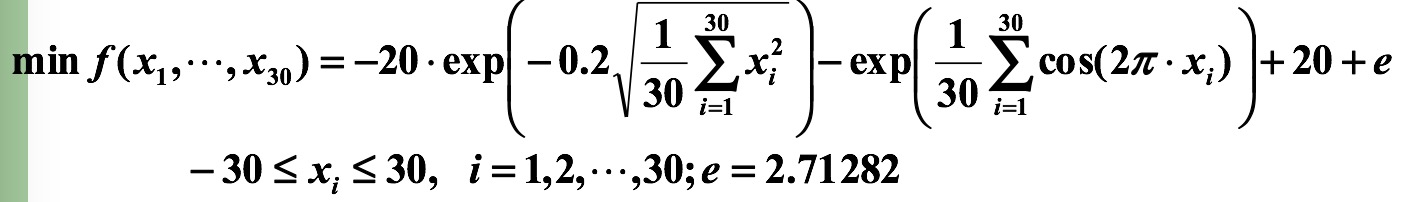
\includegraphics[width=0.8\textwidth]{algorithm.jpg}
		
		\item<2-> 求解该问题的演化策略设计如下:
		  \begin{itemize}
		     \item<1-> 表示
		\\
		       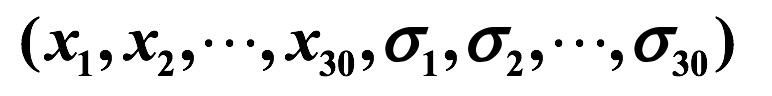
\includegraphics[width=0.8\textwidth]{algorithm2.jpg}
		     \item<2-> 适应函数:适应函数取为目标函数。
		     \item<3-> 重组算子:对变量部分使用离散重组,对策略参数部分使用全局中值重组。 
		     \item<4-> 存活选择:使用($\mu$,$\lambda$)选择,其中$\mu$=30,$\lambda$)=200。
		     \item<5-> 终止准则:当进行200000次函数值计算或发现最优解后终止算法。
		     \item<6-> 种群初始化:初始种群中每个个体的变量部分随机地产生,每个分量均匀地分布在区间       内。每个个体的变异步长都相同,设为$\theta$=3。  
	
	      \end{itemize}
		\item<3-> 运行上述算法10次,每次找到的最好解都位于全局最优峰上。

		
	\end{itemize}


   

}





%end
